\documentclass[preprint, 3p,
authoryear]{elsarticle} %review=doublespace preprint=single 5p=2 column
%%% Begin My package additions %%%%%%%%%%%%%%%%%%%

\usepackage[hyphens]{url}

  \journal{Transport Geography?} % Sets Journal name

\usepackage{graphicx}
%%%%%%%%%%%%%%%% end my additions to header

\usepackage[T1]{fontenc}
\usepackage{lmodern}
\usepackage{amssymb,amsmath}
% TODO: Currently lineno needs to be loaded after amsmath because of conflict
% https://github.com/latex-lineno/lineno/issues/5
\usepackage{lineno} % add
\usepackage{ifxetex,ifluatex}
\usepackage{fixltx2e} % provides \textsubscript
% use upquote if available, for straight quotes in verbatim environments
\IfFileExists{upquote.sty}{\usepackage{upquote}}{}
\ifnum 0\ifxetex 1\fi\ifluatex 1\fi=0 % if pdftex
  \usepackage[utf8]{inputenc}
\else % if luatex or xelatex
  \usepackage{fontspec}
  \ifxetex
    \usepackage{xltxtra,xunicode}
  \fi
  \defaultfontfeatures{Mapping=tex-text,Scale=MatchLowercase}
  \newcommand{\euro}{€}
\fi
% use microtype if available
\IfFileExists{microtype.sty}{\usepackage{microtype}}{}
\usepackage[]{natbib}
\bibliographystyle{plainnat}

\usepackage{graphicx}
\ifxetex
  \usepackage[setpagesize=false, % page size defined by xetex
              unicode=false, % unicode breaks when used with xetex
              xetex]{hyperref}
\else
  \usepackage[unicode=true]{hyperref}
\fi
\hypersetup{breaklinks=true,
            bookmarks=true,
            pdfauthor={},
            pdftitle={Leveraging GTFS to explore spatial patterns in transit supply with respect to social needs},
            colorlinks=false,
            urlcolor=blue,
            linkcolor=magenta,
            pdfborder={0 0 0}}

\setcounter{secnumdepth}{5}
% Pandoc toggle for numbering sections (defaults to be off)


% tightlist command for lists without linebreak
\providecommand{\tightlist}{%
  \setlength{\itemsep}{0pt}\setlength{\parskip}{0pt}}




\usepackage{subfig}
\usepackage{booktabs}
\usepackage{longtable}
\usepackage{array}
\usepackage{multirow}
\usepackage{wrapfig}
\usepackage{float}
\usepackage{colortbl}
\usepackage{pdflscape}
\usepackage{tabu}
\usepackage{threeparttable}
\usepackage{threeparttablex}
\usepackage[normalem]{ulem}
\usepackage{makecell}
\usepackage{xcolor}



\begin{document}


\begin{frontmatter}

  \title{Leveraging GTFS to explore spatial patterns in transit supply
with respect to social needs}
    \author[Public Transport Research Group (PTRG)]{James Reynolds%
  \corref{cor1}%
  \fnref{1}}
   \ead{james.reynolds@monash.edu} 
    \author[Public Transport Research Group (PTRG)]{Yanda Qu%
  %
  \fnref{2}}
   \ead{yanda.qu@monash.edu} 
    \author[Public Transport Research Group (PTRG)]{Graham Currie%
  %
  \fnref{3}}
   \ead{graham.currie@monash.edu} 
      \affiliation[Public Transport Research Group (PTRG)]{
    organization={Public Transport Research Group (PTRG), Institute of
Transport Studies, Department of Civil Engineering Engineering, Monash
University},addressline={Clayton
Campus},city={Melbourne},postcode={3800},state={Victoria},country={Australia},}
    \cortext[cor1]{Corresponding author}
    \fntext[1]{Research Fellow}
    \fntext[2]{PhD Strudent}
    \fntext[3]{Professor}
  
  \begin{abstract}
  This is the abstract.

  It consists of two paragraphs.
  \end{abstract}
    \begin{keyword}
    keyword1 \sep 
    keyword2
  \end{keyword}
  
 \end{frontmatter}

\hypertarget{introduction}{%
\section{Introduction}\label{introduction}}

\citet{currie2010identifying} introduced a transit Supply Index (SI) and
demonstrated how it could be used to assess spatial gaps between the
social need for public transport and what is supplied. The SI is based
on calculating a score, for each area of interest, based on the rate of
transit arrivals at nearby stops, adjusted for the amount of each area
that is within a typical walking distance. \citet{currie2010identifying}
calculated scores for areas within Greater Melbourne in Victoria,
Australia, combined these with census data to map locations with very
high social needs for transit but very low or zero supply.

Unfortunately, this approach does not appear to have been widely used,
perhaps in part because at the time it was first published the transit
Supply Index (SI) was not easy to calculate. The
\citet{currie2010identifying} analysis was based on combining multiple
operator databases and service frequency data that had been manually
extracted from transit agency websites.

Nowadays, however, the General Transit Feed Specification (GTFS) allows
timetable data to be published in a standardized format, and more than
10,000 agencies provide feeds\citep{GTFS}. Tools for analysing GTFS data
are widely available, but there is a gap as there is not yet a tool to
calculate SI scores directly from GTFS datasets. It is also unclear
whether the gaps between social needs and transit supply identified in
\citet{currie2010identifying} in Greater Melbourne have gotten better in
the almost two decades since the original analysis. Nor is it clear
whether the spatial patterns of transit need, supply and gap in
Melbourne are representative of other cities.

This provides the motivation for the research reported in this paper, in
which a new R package (gtfssupplyindex) specifically developed to
calculate SI scores is presented. The paper also reports results for
Greater Melbourne in 2016 and 2021, matching the most recent censuses
and allowing comparison to the 2006 result reported in
\citet{currie2010identifying}. Comparisons are also made to other parts
of Australia, so as to explore whether findings about Greater Melbourne
can be confidently generalized to other places.

The remainder of this paper is structured as follows: the next section
outlines the background to this research, including the original
formulation of the Transit Supply Index, and an explanation of the GTFS.
Section 3 then describes the study methodology, followed by presentation
of results in Section 4. Section 5 discusses the results and the
limitations of this stud, and outlines directions for future research. A
brief conclusion is provided in Section 6.

\hypertarget{background}{%
\section{Background}\label{background}}

\hypertarget{transit-metrics}{%
\subsection{Transit metrics}\label{transit-metrics}}

Even a brief search reveals many metrics available for benchmarking
transit services. Examples include: (1) those in the Transit Cooperative
Research Program (TCRP) Report 88, which is an extensive guidebook on
developing a performance-measurement system \citep{Ryus:2003aa}; (2)
online databases provided by the Florida Transit Information System
(FTIS) \citep{Florida-Transit-Information-System:2018aa} and
\citet{UITP:2015aa}; (3) those used in the extensive annual benchmarking
program undertaken yearly by the Transport Strategy Centre in the United
Kingdom, including over 100 transit providers around the world
\citep{Imperial-College-London:2023aa}; and (4) a recently developed
methodology to calculate `blank spots', beyond typical walking access
distances to/from transit stops\citep{AlamriSultan2023GAoA}.

The Fielding Triangle \citep{FieldingGordonJ1987Mpts} provides a
framework for combining indicators of service inputs, outputs and
consumption to describe cost efficiency, cost effectiveness and service
effectiveness. More broadly:

\begin{itemize}
\item
  \citet{Litman:2003ab} and \citet{Litman:2016aa} discuss some of the
  traffic, mobility, accessibility, social equity, strategic planning
  and other rational decision-making-based perspectives underling
  transport indicators;
\item
  \citet{Reynolds:2017ah} extends these into models of how
  institutionalism, incrementalism and other public policy analysis
  concepts might apply to decision-making processes relating to transit
  prioritization;
\item
  \citet{GuzmanLuisA.2017Aeit}, developed a measure of accessibility in
  the context of policy development and social equity for Latin American
  Bus Rapid Transit (BRT) networks; and
\item
  \citet{Creutzig2020streetspaceallocation} introduced street space
  allocation metrics based around 10 ethical principles
\end{itemize}

However, many transit metrics may be difficult to calculate, complex to
explain or understand, and likely not well suited to communication with
those who are not planners, engineers or other technical specialists.
Where pre-calculated metrics are immediately available it may not be
possible for practitioners, researchers or advocates to independently
generate scores so as to test proposed system changes. Sometimes it is
not even possible to know precisely how scores for the existing services
levels are calculated. The Transit Score metric, which is readily
available on the \citet{WalkScore:2023tg} website, provides an example.
It is available for locations with a published GTFS feed, eliminating
the need for any calculations. The meaning of these Transit Scores also
appears easy to explain, with the highest possible score of 100
representing what might be experienced in the center of New York.
However, the Transit Score algorithm is unpublished, and effectively a
black box. It does not appear that Transit Scores can be calculated
independently or generated for proposed changes to networks.

A contrasting example is the Transit Capacity and Quality of Service
Manual (TCQSM), which provides a wealth of metrics for measuring
different aspects of a transit system. The TCQSM scores themselves are
easy to understand or explain, ranging from A to F, although the number
of metrics is very large, which might limit the practicality of using
the TCQSM in practice for communicating wiht non-technical audiences.
All of these can be calculated independently, given sufficient data, and
\citet{Wong:2013aa} provides an example reporting various TCQSM metrics
across 50 transit operators. The \citet{Wong:2013aa} analysis is made
possible by the availability of General Transit Feed Specification
(GTFS) datasets for each of the transit systems

The GTFS is an open, text-based format, developed originally to allow
transit to be included in the Google Maps navigation platform
\citep{GTFS}. Figure @ref(fig:GTFS\_ERD) shows an Entity Relationship
Diagram (ERD) of the GTFS data structure. This indicates how GTFS data
is stored as a series of tables (agency, routes, trips etc.) with
primary and foreign keys (agency\_id, route\_id, trip\_id etc.)
providing links.

\begin{figure}
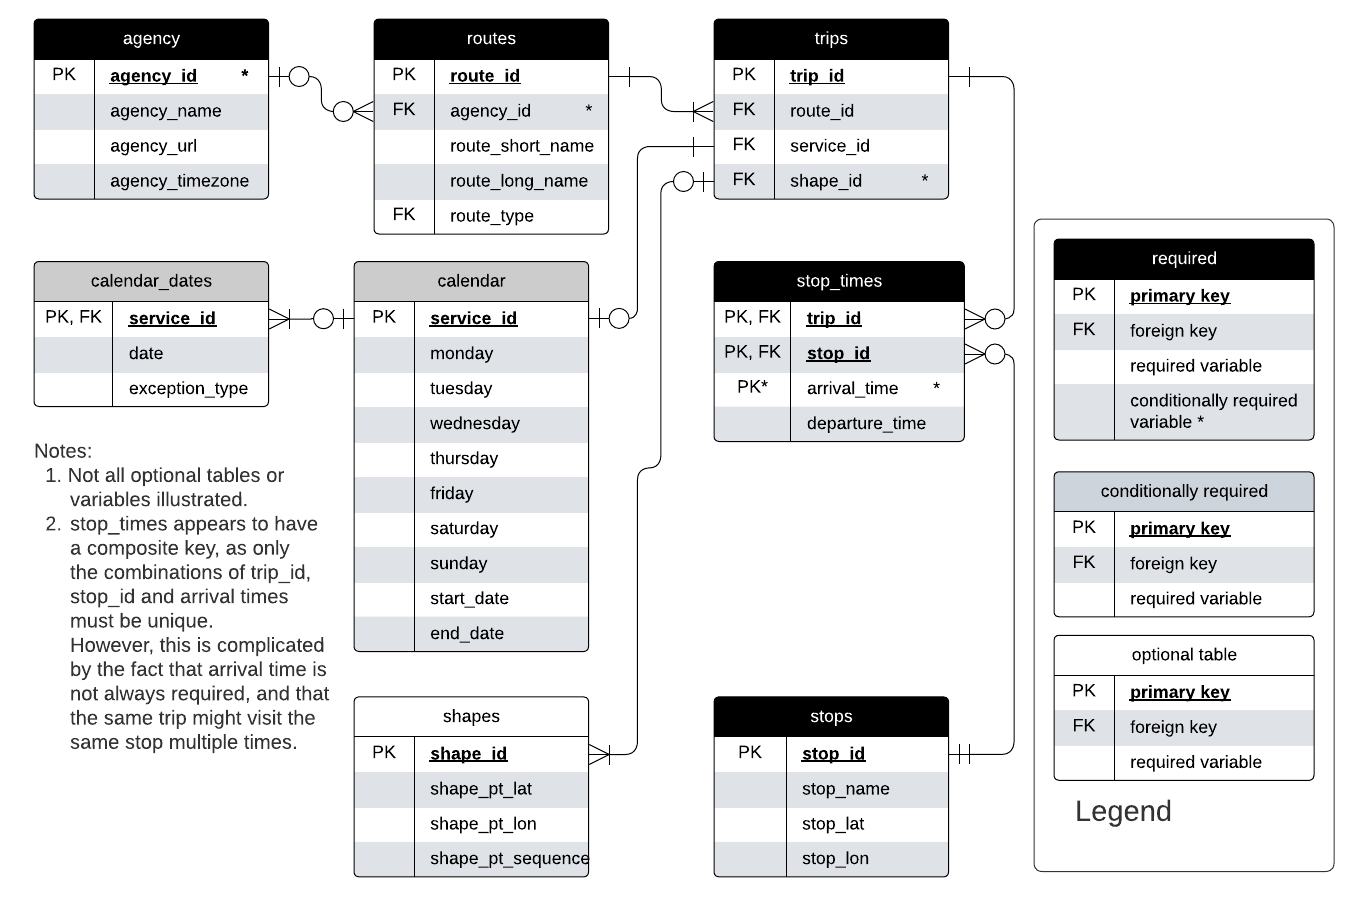
\includegraphics[width=1\linewidth]{graphics/GTFS} \caption{GTFS entity relationship diagram. Source: adapted by author from Alamri et al (2023) and the GTFS Schedule Reference (16/11/2023 revision).}\label{fig:GTFS_ERD}
\end{figure}

GTFS software tools are available for performing various analyses,
creating visulizations or other purposes. However, software to calculate
the Transit Suppy Index (SI) is not yet available.

\hypertarget{the-transit-suppy-index}{%
\subsection{The Transit Suppy Index}\label{the-transit-suppy-index}}

A generalized form of the SI equation , adapted from
\citet{currie2010identifying}, is:

\[SI_{area, time} = \sum{\frac{Area_{Bn}}{Area_{area}}*SL_{n, time}}\]

where: (1) \(SI_{area, time}\) is the Supply Index for the area of
interest and a given period of time; (2) \(Area_{Bn}\) is the buffer
area for each stop (n) within the area of interest. In
\citet{currie2010identifying} this was based on a radius of 400 metres
for bus and tram stops, and 800 metres for railway stations; (3)
\(Area_{area}\) is the area of the area of interest; and (4)
\(SL_{n,time}\) is the number of transit arrivals for each stop for a
given time period.

The SI is additive, in that \(SI_{area, time}\) scores can be aggregated
to calculate an overall score across multiple time periods or for a
region encompassing multiple areas of interest.

\begin{figure}
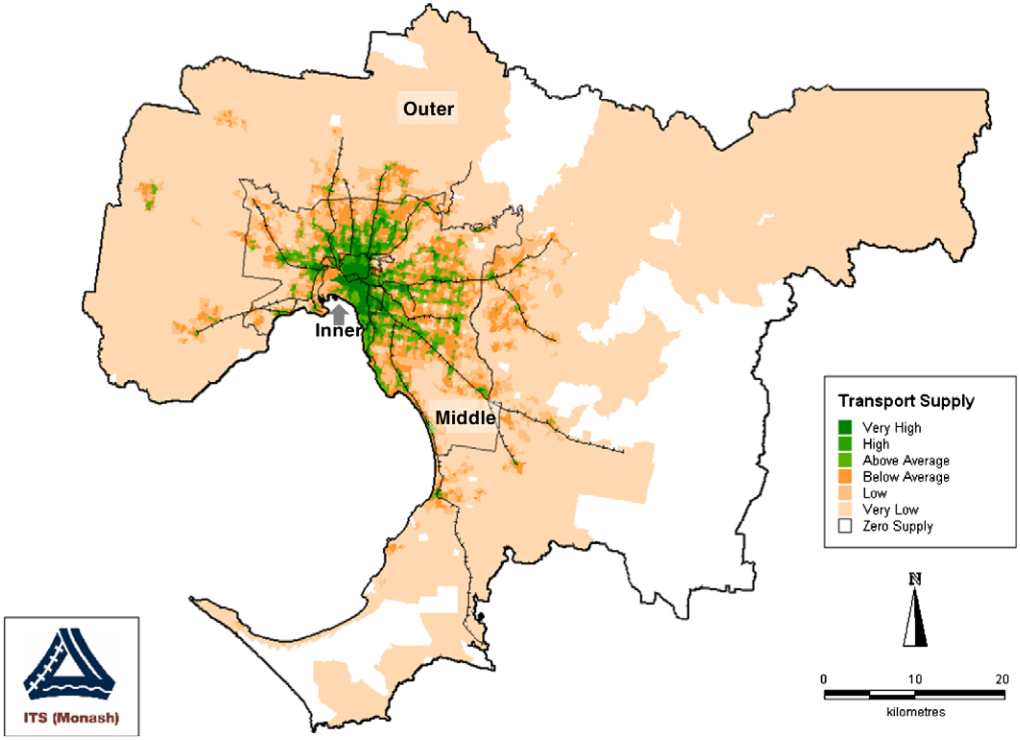
\includegraphics[width=1\linewidth]{graphics/Currie2010SI} \caption{Distribution of supply measure scores – Metropolitan Melbourne (2006), Source: Currie (2010)}\label{fig:Currie_map_SI}
\end{figure}

\begin{figure}
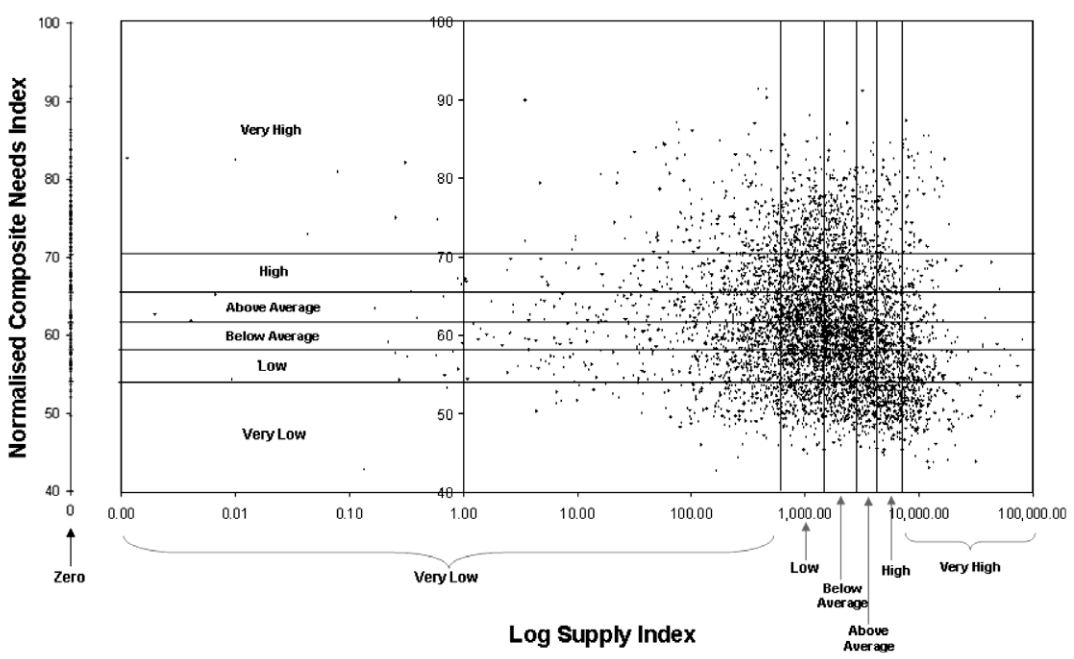
\includegraphics[width=1\linewidth]{graphics/Currie2010chart} \caption{Log supply score and need index values – Melbourne needs-gap study, Source: Currie (2010)}\label{fig:Currie_chart_gap}
\end{figure}

\begin{figure}
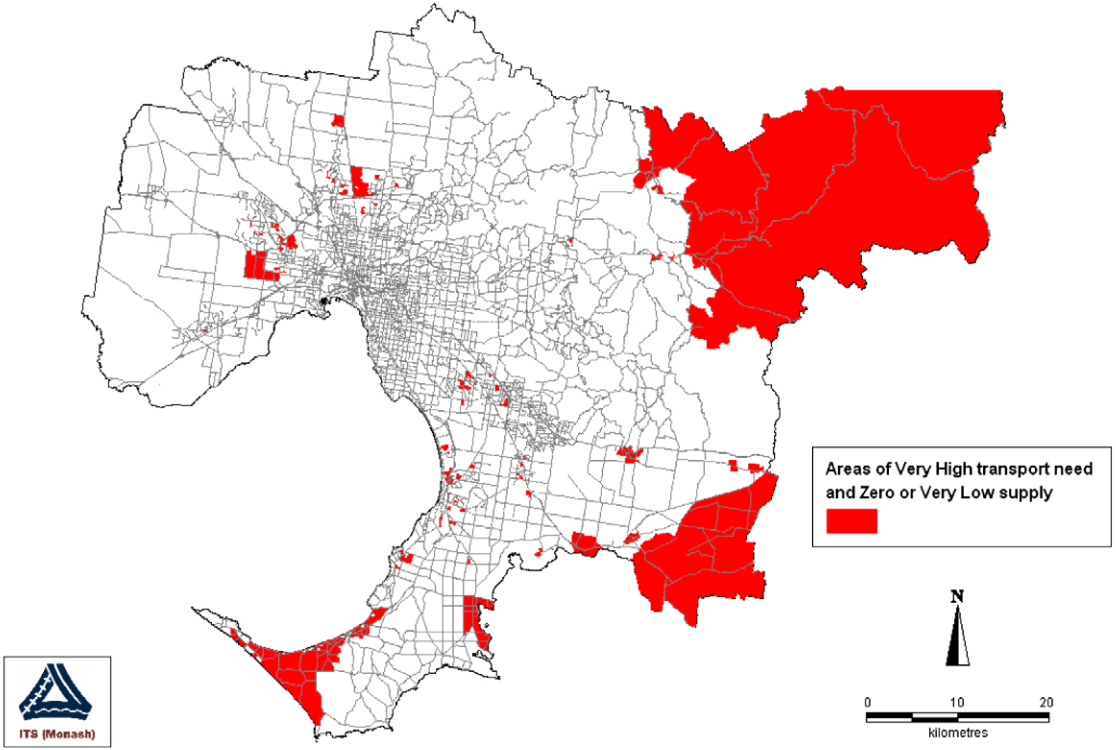
\includegraphics[width=1\linewidth]{graphics/Currie2010gap} \caption{Melbourne needs-gap – very high transport need areas with zero or very low public transport supply, Source: Currie (2010)}\label{fig:Currie_map_gap}
\end{figure}

\citet{currie2010identifying} presented maps of SI scores and areas with
very high social needs but zero or very low transit supply, and a chart
contrasting needs and supply (see Figures \ref{fig:Currie_map_SI},
\ref{fig:Currie_chart_gap} and \ref{fig:Currie_map_gap}. However, it
doesn't appear that there have been similar analyses undertaken since
then, so it is unclear whether gaps between transit needs and supply
have improved, remained similar or become worse. Nor does it appear that
this methodology has been applied to other places, except for similar
studies of Hobart and Adelaide discussed in
\citet{currie2010identifying}. Hence, it is unclear whether the patterns
in Melbourne, where areas with very high transport needs but zero or
very low transit supply tend to be in middle and outer areas of the city
serviced by buses, is consistent with patterns in other cities.
Comparing current conditions and other locations to the findings of
\citet{currie2010identifying}, therefore, is an aim of the research
discussed in this paper.

\hypertarget{methodology}{%
\section{Methodology}\label{methodology}}

This study developed a package with tools for calculating the SI from
GTFS data. The R programming language \citep{R-base} was adopted for
code development. Package development setup and workflow as described by
\citet{wickham2023r} was adopted. Various existing packages were relied
upon including: the sf package \citep{R-sf} for geospatial analysis; the
tidyverse \citep{tidyverse2019}; gtfstools \citep{R-gtfstools}; and
tidytransit \citep{R-tidytransit}. Some code was adapted from examples,
vignettes and other documentation in the tidytransit, gtfstools and
other packages.

Two cases where used during the code development and testing, such that
results might be generated for real GTFS data: the Mornington Peninsula
Tourist Railway GTFS feed and the Public Transport Victoria (PTV) GTFS
feed, both in Victoria, Australia. Both were selected primarily for
convenience, given that the authors are familiar with the typical
service patterns and geography. The Mornington Peninsula Tourist Railway
network, consisting of only three stations, also facilitated hand
calculation of the SI as a cross-check of the results produced by the
developed package.

Figure @ref(Melbourne\_map)) shows the areas of interest relevant to the
code development and testing, and selected railway stations. Statistical
Area (SA) zones from the Australian Bureau of Statistics \citep{ABSmaps}
Areas of interest included Greater Melbourne (main) and SA1 zones within
800 metres of the Mornington Penninsula railway (right). SA1 zones are
the smallest geographical areas for which results are reported in the
Australian census, while the main image of Figure @ref(Melbourne\_map))
shows the boundary of the Greater Melbourne Greater Capital City (GCC)
zone and SA3 zone boundaries, which are generally similar to Local
Government Area (LGA) boundaries (albeit with some LGAs split into two
zones).

\begin{figure}
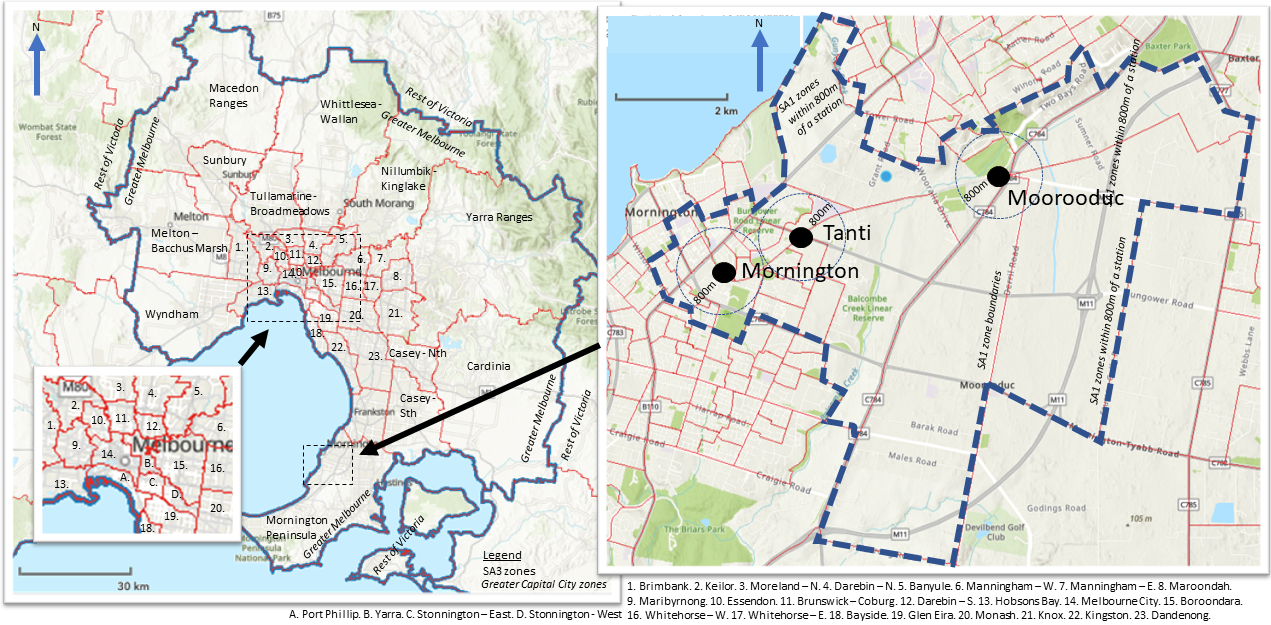
\includegraphics[width=1\linewidth]{graphics/all_maps} \caption{Areas of interest}\label{fig:Melbourne_map}
\end{figure}

\hypertarget{mornington-penninsula-tourist-railway}{%
\subsection{Mornington Penninsula Tourist
Railway}\label{mornington-penninsula-tourist-railway}}

The Morning Peninsula Tourist Railway is in the outer south-east of
Melbourne, running on Sundays and Wednesdays between Mornington and
Moorooduc, with an intermediate stop at Tanti Park (see
https://transitfeeds.com/p/mornington-railway/806/latest/stops). A GTFS
feed from 2018 was selected for the purposes of tests and demonstrating
the code and output. Australian Bureau of Statistics (ABS) data was also
used, sources via the strayr and absmapsdata packages \citep{r-strayr}.
The Mornington Peninsular Statistical Area 3 (SA3) zone and the
Statistical Area 1 (SA1) zones contained within it were adopted as the
areas of interest.

\hypertarget{public-transport-victoria-ptv}{%
\subsection{Public Transport Victoria
(PTV)}\label{public-transport-victoria-ptv}}

The Victorian GTFS feed, published by Public Transport Victoria (PTV)
and with historical feeds sourced via
\citet{transitfeeds_victoria:2023aa}, was used for analysis of Victoria.
SI scores were obtained for the weeks starting on the day of the census
in 2016 and 2021, which were on Tuesday 9th and 10th of August
respectively.

\hypertarget{results}{%
\section{Results}\label{results}}

\hypertarget{code-structure-and-functionality}{%
\subsection{Code structure and
functionality}\label{code-structure-and-functionality}}

Developed code is available and documented on github
\citep{gtfssupplyindex_github}. The structure of the package, functions
developed, and data tables are shown in Figure @ref(fig:SI\_ERD). This
shows\\
how the package takes input from three files: a gtfs feed (gtfs.zip); a
sf object describing the geometry of the areas for which the SI is to be
calculated; and a csv file (included in the package) defining the buffer
zone distances for each route type. The ultimate output is a
si\_by\_area\_and\_hour table (bottom-right), which reports the SI score
for each hour of the day across dates specified by the user.

\begin{figure}
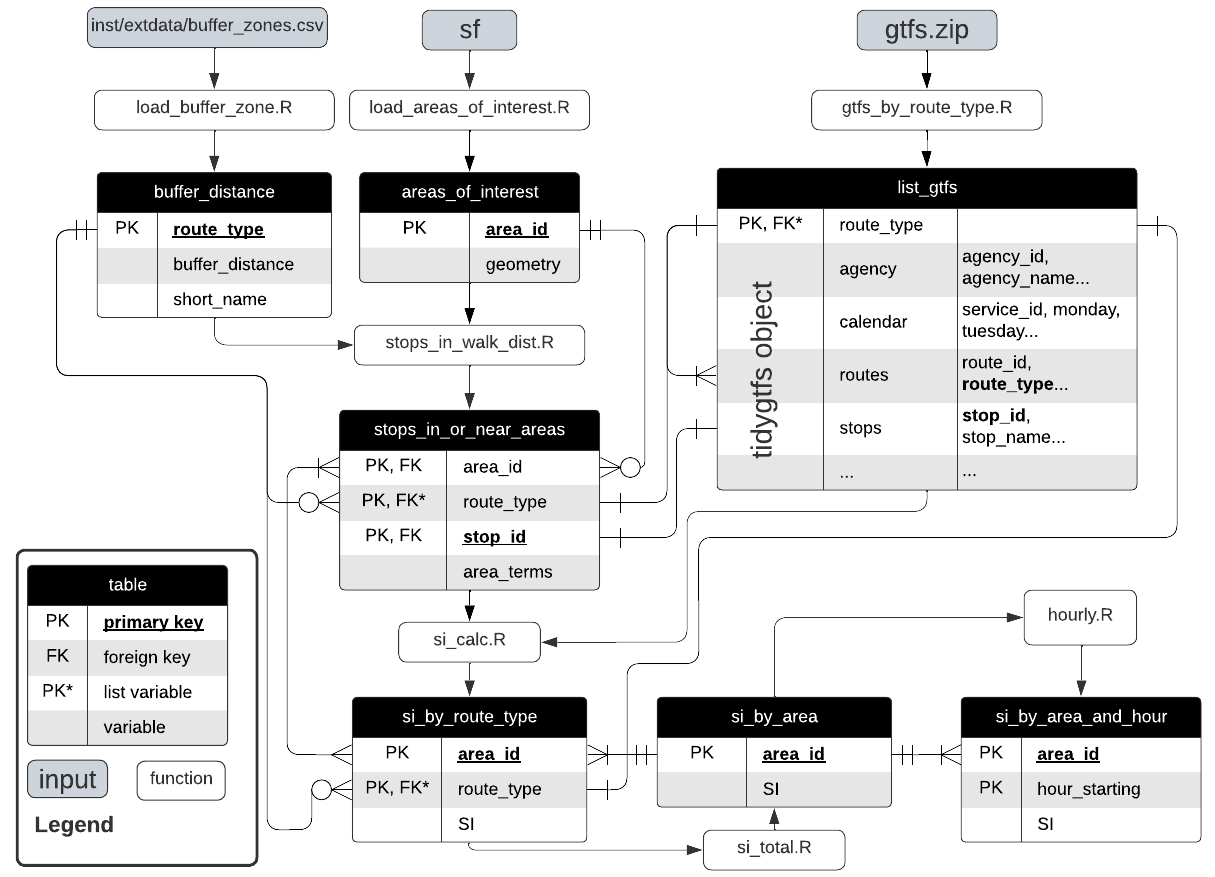
\includegraphics[width=1\linewidth]{graphics/SI_data_structure} \caption{Entity Relationship Diagram (ERD) showing the data structure and functions related to the gtfssupplyindex package}\label{fig:SI_ERD}
\end{figure}

Various functions and their output are explained in the following, using
the Mornington Peninsula GTFS for December 30th, 2018, and SA1 zone
boundaries as a worked example. Individual steps are:

\begin{enumerate}
\def\labelenumi{(\arabic{enumi})}
\item
  loading the gtfs.zip file: the gtfs\_by\_route\_type function loads
  the gtfs data and splits it into a list (by route\_type) of tidygtfs
  objects, using the filter\_by\_route\_type function from the gtfstools
  package \citep{filter_GTFS_by_mode}.
\item
  loading geometry information about the areas of interest: geographical
  data about the areas of interest are loaded by the
  load\_areas\_of\_interest.R function into an sf object, using the sf
  package \citep{R-sf}. The resultant areas\_of\_interest table contains
  each area\_id and its associated geometry. Data about buffer zones,
  specifically the walking distance threshold assigned to each
  route\_type (mode) is then loaded, again through a function
  (load\_buffer\_zone.R).
\item
  calculating which stops are within the catchment walking distance of
  which areas: using the stops\_in\_walk\_dist function. Figure
  @ref(fig:calculate\_stop\_in\_or\_near\_areas\_verbose)) shows how
  this function identified SA1 areas within the 800 metre catchment of
  the three Mornington stations.
\end{enumerate}

\begin{figure}
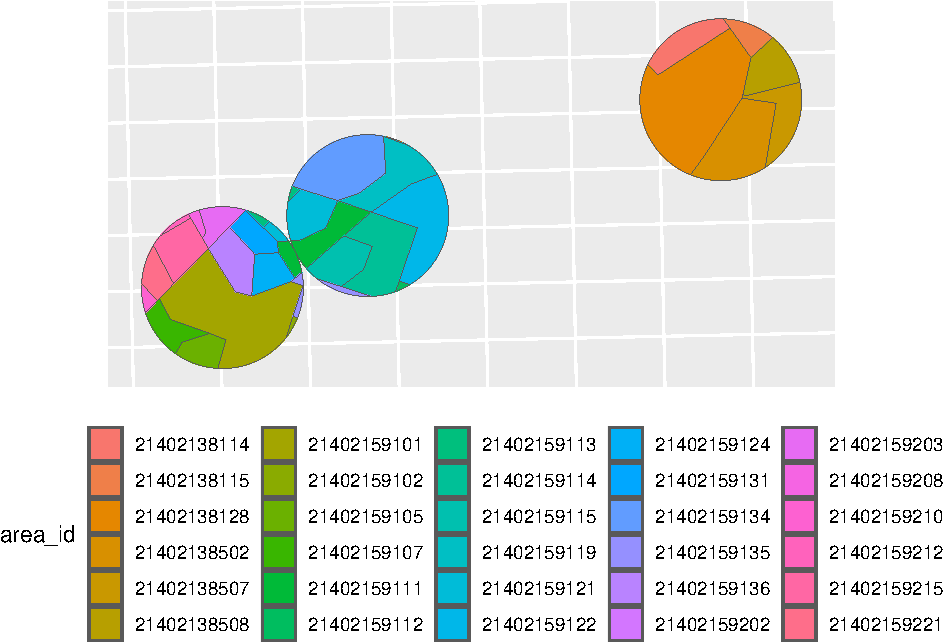
\includegraphics[width=1\linewidth]{Leveraging_GTFS_to_assess_transit_supply_Transport_Geography_files/figure-latex/calculate_stop_in_or_near_areas_verbose-1} \caption{Step 3, stop catchments for the Mornington Penninsula Tourist Railway, showing intersections with SA1 zones}\label{fig:calculate_stop_in_or_near_areas_verbose}
\end{figure}

\begin{enumerate}
\def\labelenumi{(\arabic{enumi})}
\setcounter{enumi}{3}
\tightlist
\item
  Calculating SI scores for a given time period: The si\_calc.R function
  calculates the number of arrivals in a given time period, using code
  adapted from an article included in the tidytransit package
  \citep{tidytransit_departure_timetable}, and combines this with the
  calculated area components. The si\_total.R and hourly.R functions
  provided aggregation, giving the results mapped in Figure
  @ref(fig:SI\_mornington\_20181230\_output).
\end{enumerate}

\begin{figure}
\centering
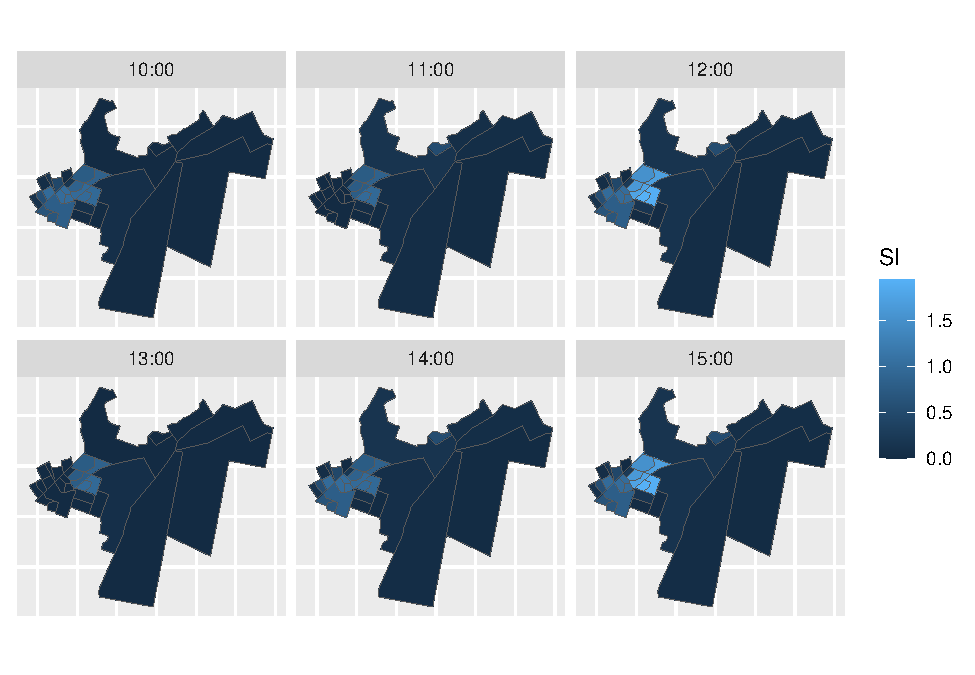
\includegraphics{Leveraging_GTFS_to_assess_transit_supply_Transport_Geography_files/figure-latex/SI_mornington_20181230_output-1.pdf}
\caption{Mornington Penninsula Tourist Railway hourly SI values for
December 30, 2018}
\end{figure}

\hypertarget{si-scores}{%
\subsection{SI scores}\label{si-scores}}

\begin{figure}
\centering
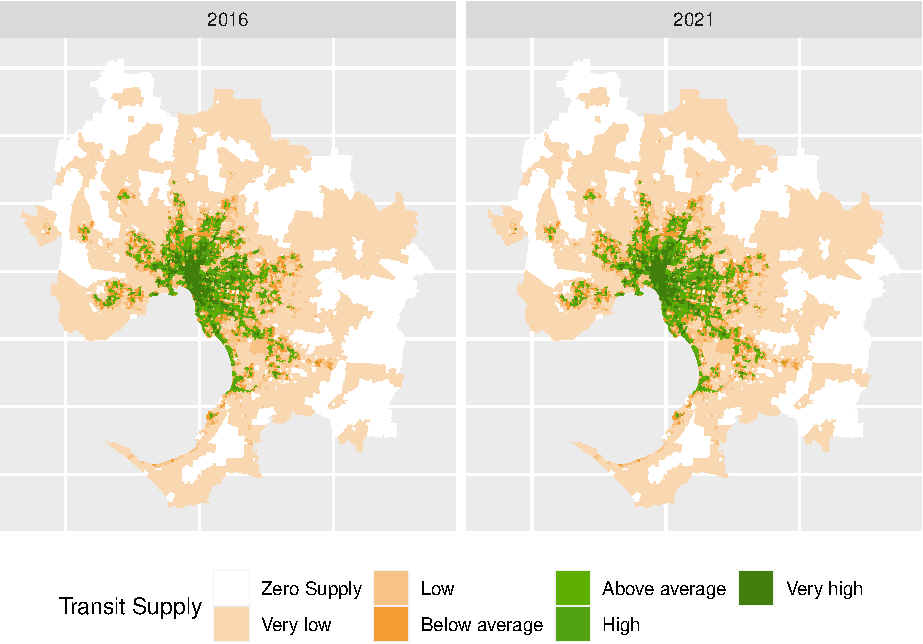
\includegraphics{Leveraging_GTFS_to_assess_transit_supply_Transport_Geography_files/figure-latex/Greater_Melbourne_2016_2021-1.pdf}
\caption{SI scores, census day 2016 and 2021}
\end{figure}

\hypertarget{imrad}{%
\subsubsection{IMRAD}\label{imrad}}

\hypertarget{comparing-cases}{%
\subsection{Comparing cases}\label{comparing-cases}}

\hypertarget{population-and-equality}{%
\subsubsection{Population and equality}\label{population-and-equality}}

\hypertarget{purpose-of-transit-in-the-citys-transport-policy}{%
\subsection{Purpose of transit in the city's transport
policy}\label{purpose-of-transit-in-the-citys-transport-policy}}

\hypertarget{indexes-and-comparing-cities}{%
\subsection{Indexes and comparing
cities}\label{indexes-and-comparing-cities}}

\hypertarget{discussion}{%
\section{Discussion}\label{discussion}}

\hypertarget{limitations-and-directions-for-furture-research}{%
\subsection{Limitations and directions for furture
research}\label{limitations-and-directions-for-furture-research}}

\hypertarget{conclusions}{%
\section{Conclusions}\label{conclusions}}

\renewcommand\refname{References}
\bibliography{References.bib, packages.bib}


\end{document}
